\section{Pilot results (development split)}
\label{sec:results}
% Numbers come from reports/pilot/results_dev.json and runs/go_no_go_rev1.json
% and reports/pilot/seeds_dev_interim.json (checked by tests/test_paper_results.py and
% tests/test_paper_seeds.py). Locked-test numbers are not typed here; they are in
% test_results.tex, generated from reports/final/ (opened 2026-11-22).

Table~\ref{tab:results-dev} lists every trained arm on the 200 development root graphs of the
pilot build, image input, strict scoring, one training seed. Intervals are 95\% root-graph
bootstrap intervals (2000 replicates); differences are paired on the same root graphs against
B trained on the same machine (Kaggle T4). These are pilot numbers on the split used for
decisions, not test results.

\begin{table}[t]
\centering\small
% Generated by scripts/results_table.py; do not edit by hand.
\begin{tabular}{lccccc}
\toprule
Arm & Repair & Reach. & Crit. edge & Non-edit macro & $\Delta$ macro vs B\_kaggle \\
\midrule
B\_kaggle & 0.292 & 0.830 & 0.762 & 0.796 & ref \\
C\_kaggle & 0.255 & 0.700 & 0.375 & 0.537 & $-0.259$ {\scriptsize[$-0.294$, $-0.224$]} \\
E\_kaggle & 0.830 & 0.935 & 0.833 & 0.884 & $+0.088$ {\scriptsize[$+0.054$, $+0.121$]} \\
B\_colab & 0.295 & 0.845 & 0.770 & 0.807 & $+0.011$ {\scriptsize[$-0.006$, $+0.028$]} \\
D\_colab & 0.545 & 0.840 & 0.502 & 0.671 & $-0.125$ {\scriptsize[$-0.153$, $-0.099$]} \\
D2\_kaggle & 0.500 & 0.770 & 0.495 & 0.633 & $-0.164$ {\scriptsize[$-0.190$, $-0.138$]} \\
\bottomrule
\end{tabular}

\caption{Development-split accuracy (pilot build, 200 root graphs, one seed). Reach.\ =
reachability, Crit.\ edge = critical edge; the non-edit macro averages these two. The last
column is the paired difference in non-edit macro accuracy to B\_kaggle with its 95\% interval.
The suffix names the machine the arm was trained on.}
\label{tab:results-dev}
\end{table}

\paragraph{Repair training does not transfer to the non-edit questions.}
Both repair-trained arms are below B on their own machine: D by $-0.136$
($-0.163$ to $-0.109$) and the revised D2 by $-0.164$ ($-0.190$ to $-0.138$) in non-edit
macro accuracy; no bootstrap replicate of either difference was above zero. Retraining B on the
second machine moved it by $-0.011$ ($-0.028$ to $+0.006$), so the gap is not a machine effect.
By the rule fixed before this comparison was read (Section~\ref{sec:negative}), the transfer
hypothesis is closed as not supported at pilot scale and the second allowed revision is not spent.

\paragraph{The structural baseline is weaker still.}
C, trained on graph description, masked infilling and graph matching over the same images, reaches
a non-edit macro of $0.537$, $-0.259$ ($-0.294$ to $-0.224$) below B. Its critical-edge
accuracy ($0.375$) is below the balanced chance level, so the structural tasks did not supply
the edge-level reasoning the questions need.

\paragraph{The gaps hold across three training seeds.}
B, C, D and the parser of E were each trained with all three pre-registered seeds on the same machine
(Kaggle T4);
Table~\ref{tab:seeds-dev} pools them. Pooling averages the seeds on the same resampled root graphs
(2000 replicates), so the interval reflects the root graphs, not seed variance; the per-seed gaps
are reported next to it. Pooled over seeds, D is $-0.131$ ($-0.153$ to $-0.110$) and C is
$-0.249$ ($-0.277$ to $-0.222$) below B in non-edit macro accuracy, and every seed-matched gap has
the same sign (D: $-0.136$ to $-0.124$; C: $-0.259$ to $-0.241$). By the rule fixed before the
second seed was read, both are negative readings. The same seed table chose B over C as the
reference baseline for the locked test. The parse-and-solve arm E, whose description parser was
retrained per seed, is $+0.072$ ($+0.042$ to $+0.102$) above B, with every seed-matched gap
positive (E: $+0.061$ to $+0.088$), a clear positive reading by the same rule: on the development
split, transcribing the drawing and solving exactly is the strongest of the four seed-pooled arms.

\begin{table}[t]
\centering\small
% Generated by scripts/seed_table.py; do not edit by hand.
\begin{tabular}{lcccccc}
\toprule
Arm & Seeds & Repair & Reach. & Crit.\ edge & Non-edit macro & $\Delta$ macro vs B \\
\midrule
B & 3 & 0.302 & 0.828 & 0.767 & 0.798 {\scriptsize[0.776, 0.822]} & ref \\
C & 3 & 0.252 & 0.689 & 0.408 & 0.549 {\scriptsize[0.530, 0.569]} & $-0.249$ {\scriptsize[$-0.277$, $-0.222$]} \\
D & 3 & 0.537 & 0.814 & 0.519 & 0.667 {\scriptsize[0.647, 0.686]} & $-0.131$ {\scriptsize[$-0.153$, $-0.110$]} \\
E & 3 & 0.838 & 0.925 & 0.814 & 0.870 {\scriptsize[0.844, 0.894]} & $+0.072$ {\scriptsize[$+0.042$, $+0.102$]} \\
\bottomrule
\end{tabular}

\caption{Development split, pooled over three training seeds (2027, 3407, 9173) per arm, all
trained on Kaggle T4. Task columns are pooled accuracy; brackets are 95\% root-graph bootstrap
intervals of the pooled value; the last column is the pooled paired difference to B.}
\label{tab:seeds-dev}
\end{table}

\begin{figure}[t]
\centering
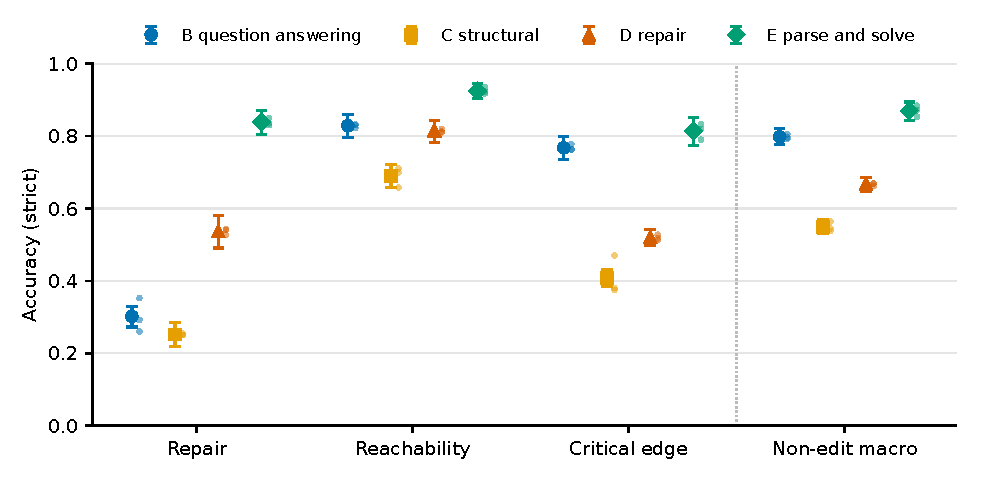
\includegraphics[width=\textwidth]{figures/arms_dev.pdf}
\caption{Development split, the values of Table~\ref{tab:seeds-dev} per task. Marker: accuracy pooled
over the three training seeds; bar: its 95\% root-graph bootstrap interval; small dots: single seeds.
The accuracy axis runs from 0 to 1. Generated from the recorded metrics by \texttt{scripts/dev\_figures.py}.}
\label{fig:arms-dev}
\end{figure}

\paragraph{Cost.}
Figure~\ref{fig:arms-dev} shows the same ordering of the pooled values on every non-edit task. The end-to-end arms cost
about the same to evaluate: on the 1200 development samples one run of B, C or D took $1128.6$ to
$1319.5$ T4 seconds. E took $4141.7$ to $4287.8$ seconds, because it writes out the whole edge list
before the solver answers; its advantage on this split is bought with more than three times the
evaluation time. Training times lie between $1487.7$ and $2079.3$ seconds for all twelve runs.

\begin{figure}[t]
\centering
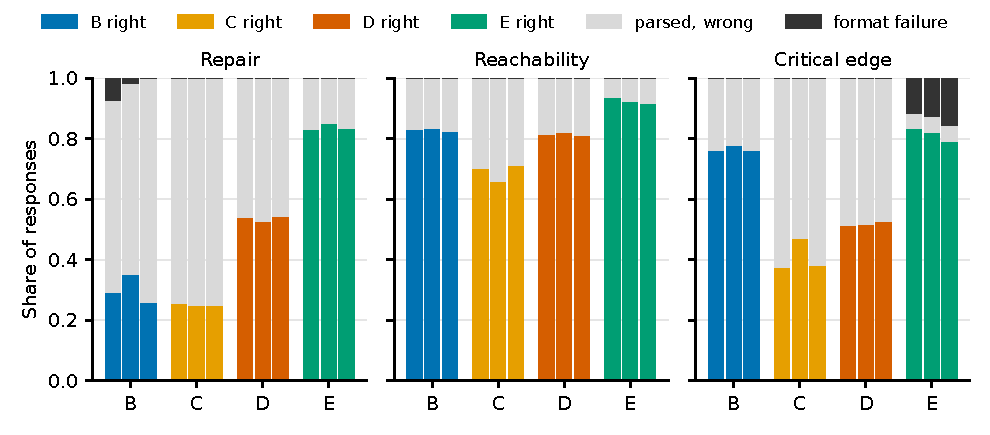
\includegraphics[width=\textwidth]{figures/errors_dev.pdf}
\caption{Development split, what the responses of each run were (one bar per training seed).
Coloured: right under the strict parser; light grey: parsed but wrong; dark: format failure, which
counts as wrong. For E a dark segment is a critical-edge question whose premise fails on the
transcribed graph, so the solver gives no answer. Accuracy and format-failure rate are the recorded
ones; the grey share is their remainder. Generated by \texttt{scripts/dev\_figures.py}.}
\label{fig:errors-dev}
\end{figure}

\paragraph{Error types.}
Figure~\ref{fig:errors-dev} splits the errors of each run. The end-to-end arms almost never fail on
format: C and D have no format failure on any task in any run, and B has none on the two non-edit
tasks and $29$, $7$ and $1$ of $400$ on repair (seeds 3407, 2027, 9173). Their errors are
well-formed wrong answers, and the recorded lenient score equals the strict one on every task in all
nine runs. E is different on one task: for $47$, $50$ and $62$ of its $400$ critical-edge questions per run
the premise fails on the transcribed graph (the source does not reach the target there, or the
queried edge is missing), the solver returns no answer, and the sample is scored as wrong.
These are $47$ of $67$, $50$ of $72$ and $62$ of $84$ of E's critical-edge errors, so most of what E loses there
is a transcription error surfacing as an unanswerable question, not a wrong computation.

\paragraph{Where repair training helps.}
On the repair task itself D ($0.545$) and D2 ($0.500$) are well above B ($0.292$) and C ($0.255$),
so the adapters did learn the training task; the failure is in the transfer.

\paragraph{Parsing the drawing and solving exactly beats every end-to-end arm.}
E uses an adapter trained only to transcribe the drawing as an edge list (same images, same
budget) and answers every question with the exact solver on the transcribed graph. It reaches a
non-edit macro of $0.884$, $+0.088$ ($+0.054$ to $+0.121$) above B, and $0.830$ on repair.
Its transcription is exact for only $359$ of $763$ development images, so the end-to-end arms do not
lose to E because the drawings are unreadable. On the samples whose image E reads exactly, D is
still $-0.148$ ($-0.190$ to $-0.105$) below B, so the gap does not come from drawings that are hard
to transcribe. The split fixed before E was read back (Section~\ref{sec:analysis}) labels this a
reasoning gap; that label uses E's parser as a proxy for how hard a drawing is and does not measure
what the other arms perceived, so it does not by itself rule out a part for perception.
